% SPDX-License-Identifier: CC-BY-SA-4.0
% Part: Introduction
% Section: Mathematical and Logical recalls
% Challenge exercise: Foundation of inductive definitions

\begingroup

\begin{exercice}[Mini-défi -- Définition inductive]\label{exo:introduction/maths/challenge}

  On cherche à définir formellement le sous-ensemble $E$ de $\mathbb{R}$ représenté graphiquement ci-dessous: 
  \begin{center}
    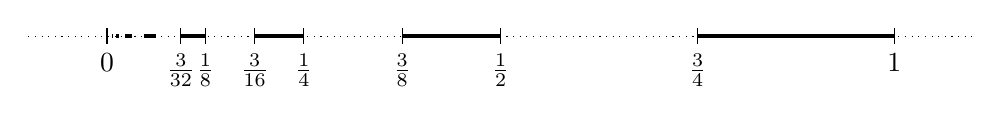
\begin{tikzpicture}
      \draw[dotted] (-1,1) -- (11,1);
      \draw[ultra thick] (7.5/1  ,1) -- (10/1  ,1);
      \draw[ultra thick] (7.5/2  ,1) -- (10/2  ,1);
      \draw[ultra thick] (7.5/4  ,1) -- (10/4  ,1);
      \draw[ultra thick] (7.5/8  ,1) -- (10/8  ,1);
      \draw[ultra thick] (7.5/16 ,1) -- (10/16 ,1);
      \draw[ultra thick] (7.5/32 ,1) -- (10/32 ,1);
      \draw[ultra thick] (7.5/64 ,1) -- (10/64 ,1);
      \draw[ultra thick] (7.5/128,1) -- (10/128,1);

      \draw (0    ,1.1) -- (0    ,0.9) node[below]{$0$};
      \draw (7.5/8,1.1) -- (7.5/8,0.9) node[below]{$\frac{3}{32}$};
      \draw (1.25 ,1.1) -- (1.25 ,0.9) node[below]{$\frac{1}{8}$};
      \draw (7.5/4,1.1) -- (7.5/4,0.9) node[below]{$\frac{3}{16}$};
      \draw (2.5  ,1.1) -- (2.5  ,0.9) node[below]{$\frac{1}{4}$};
      \draw (7.5/2,1.1) -- (7.5/2,0.9) node[below]{$\frac{3}{8}$};
      \draw (5    ,1.1) -- (5    ,0.9) node[below]{$\frac{1}{2}$};
      \draw (7.5  ,1.1) -- (7.5  ,0.9) node[below]{$\frac{3}{4}$};
      \draw (10   ,1.1) -- (10   ,0.9) node[below]{$1$};
    \end{tikzpicture}
  \end{center}

  On commence par remarquer que $E$ vérifie l'équation (\ref{equation:introduction/maths/inductive_defs}) ci-dessous :
  \begin{equation}\label{equation:introduction/maths/inductive_defs}
    \left[\frac{3}{4} , 1\right] \subseteq E
    \quad\land\quad
    \forall x \in E,  \frac{x}{2} \in E
  \end{equation}
    
  Soit $\displaystyle \mathcal{S} \eqdef \left\{X\in \mathscr{P}(\mathbb{R}) \,\middle|\, \left[\frac{3}{4} , 1\right] \subseteq X \land \forall x \in X, \frac{x}{2} \in X\right\} $
  l'ensemble des solutions de l'équation (\ref{equation:introduction/maths/inductive_defs}). 
  
  \begin{question}
  \item Montrer que $\mathbb{R} \in \mathcal{S}$, $[0, 1] \in \mathcal{S}$ et $\left[0, \frac{1}{2}\right] \cup \left[\frac{3}{4} , 1\right] \in \mathcal{S}$.
  \item Montrer que $\forall X \in \mathcal{S}, \forall X' \in \mathcal{S}, X \cap X' \in \mathcal{S}$.
  \end{question}

  On définit $E$ comme la plus petite des solutions au sens de l'inclusion :
  $$E \eqdef \bigcap_{X\in \mathcal{S}} X = \{x \in \mathbb{R} \mid \forall X \in \mathcal{S}, x \in X\}.$$

  \begin{question}
  \item Montrer que $1 \in E$ et que $\frac{1}{2} \in E$.
  \item Montrer que $2 \notin E$ et que $\frac{2}{3} \notin E$.
  \item Montrer que $\forall x < 1, x\notin E \Rightarrow \frac{x}{2} \notin E$.
    %  \item Montrer que $\forall X \in \mathscr{P}(\mathbb{R}), ([\frac{3}{4}, 1] \subseteq X \land \forall x \in X, \frac{x}{2} \in X) \implies E \subseteq X$
  \end{question}

  On pose maintenant le prédicat suivant : $P(x) \eqdef \exists y \in \mathbb{R}, 0 < y < x \land  y\notin E$.\\
  On cherche à démontrer $\forall x\in E, P(x)$ \emph{par induction sur $x$}.
  \begin{question}
  \item Montrer que $\forall x \in \left[\frac{3}{4}, 1\right], P(x)$.
  \item Montrer que $\forall x \in E, P(x) \Rightarrow P\left(\frac{x}{2}\right)$.
  \item Montrer que $\forall x\in E, P(x)$.
  \end{question}

\end{exercice}

\begin{correction}

  \begin{question}
  \item Il y a à chaque fois deux choses à vérifier :
    \begin{itemize}
    \item $[\frac{3}{4} , 1] \subseteq \mathbb{R} \subseteq \mathbb{R}$, et $\forall x \in \mathbb{R}, \frac{x}{2} \in \mathbb{R}$.
    \item $[\frac{3}{4} , 1] \subseteq [0, 1] \subseteq \mathbb{R}$, et $\forall x \in [0, 1], \frac{x}{2} \in [0, 1]$.
    \item $[\frac{3}{4} , 1] \subseteq [0, \frac{1}{2}] \cup [\frac{3}{4} , 1] \subseteq \mathbb{R}$, et $\forall x \in [0, \frac{1}{2}] \cup [\frac{3}{4} , 1], \frac{x}{2} \in [0, \frac{1}{2}] \subseteq [0, \frac{1}{2}] \cup [\frac{3}{4} , 1]$.
    \end{itemize}
  \item Soient $X, X' \in \mathcal{S}$.
    \begin{itemize}
    \item $X \in \mathscr{P}(\mathbb{R})$ et $X' \in \mathscr{P}(\mathbb{R})$, donc $X \cap X' \in \mathscr{P}(\mathbb{R})$.
    \item Soit $x \in [\frac{3}{4} , 1]$. On a $x\in X$ et $x \in X'$, donc $x \in X\cap X'$.
    \item Soit $x \in X\cap X'$. Montrons que $\frac{x}{2} \in X \cap X'$.\\
      Comme $x \in X$ et $X \in \mathcal{S}$, $\frac{x}{2} \in X$. De même, $\frac{x}{2} \in X'$. Donc $\frac{x}{2} \in X \cap X'$. 
    \end{itemize}
    Finalement, $X \cap X' \in \mathcal{S}$.
  \item On revient à la définition $x \in \mathbb{R} \land (\forall X \in \mathcal{S}, x \in X) \Rightarrow x \in E$. 
    \begin{itemize}
    \item Soit $X \in \mathcal{S}$. On a $1 \in [\frac{3}{4} , 1] \subseteq X$. On a donc, $1 \in \mathbb{R} \land \forall X \in \mathcal{S}, x \in X$, donc $1\in E$. 
    \item Pour tout $X \in \mathcal{S}$, $1 \in X$, donc $\frac{1}{2} \in X$. Donc $\frac{1}{2} \in E$.
    \end{itemize}
  \item Par définition, $x \in E \Rightarrow \forall X \in \mathcal{S}, x \in X$. On prend la contraposée $(\exists X \in \mathcal{S}, x \notin X) \Rightarrow x\notin E$. 
    \begin{itemize}
    \item $[0,1] \in \mathcal{S}$ et $2\notin [0,1]$, donc $2 \notin E$. 
    \item $[0, \frac{1}{2}] \cup [\frac{3}{4} , 1] \in \mathcal{S}$ et $\frac{2}{3}\notin [0, \frac{1}{2}] \cup [\frac{3}{4} , 1]$, donc $\frac{2}{3} \notin E$. 
    \end{itemize}
  \item Supposons, (par l'absurde), qu'il existe $x<1$ tel que $x\notin E$ et $\frac{x}{2} \in E$.
    Posons $F = E \setminus \{\frac{x}{2}\}$.  
    \begin{enumerate}
    \item Montrons que $F \in \mathcal{S}$. 
      \begin{itemize}
      \item On a bien $F \subseteq E \subseteq \mathbb{R}$.
      \item Soit $y \in [\frac{3}{4}, 1]$. On a bien $y\in E$. De plus, $y > \frac{1}{2}$, donc $y \neq \frac{x}{2}$, donc $y\in F$. 
      \item Soit $y \in F$. Alors $y\in E$, donc $\frac{y}{2} \in E$. De plus, $\frac{y}{2} \neq \frac{x}{2}$ puisque $x\notin E$. Donc $\frac{y}{2}\in F$. 
      \end{itemize}
    \item $F \in \mathcal{S}$ et $\frac{x}{2} \notin F$, donc $\frac{x}{2} \notin E$. Absurde. 
    \end{enumerate}
  \item Soit $x \in \left[\frac{3}{4}, 1\right]$. On a $0 < \frac{2}{3} < x$ et $\frac{2}{3} \notin E$. 
  \item Soit $x \in E$ tel que $P(x)$, et soit $y$ donné par $P(x)$, tel que $0 < y < x$ et $y\notin E$.
    On a $0 < \frac{y}{2} < \frac{x}{2}$ et $\frac{y}{2}\notin E$. 
  \item Posons $X \eqdef \{x\in E | P(x)\}$. D'après les deux points précédents,
    on a $X\in \mathcal{S}$, donc $E \subseteq X$. \\
    Soit $x \in E$. On a $x\in X$, donc $P(x)$.  
  \end{question}

\end{correction}

\endgroup
\endinput
